\section{Challenges and Opportunities}\label{sec:challenges}

What becomes a challenge is when all branches of a PHYSLITE file need to be read including branches with custom objects and when systematics need to be handled.
As columnar analysis processes events in batches, this requires that ATLAS Combined Performance (CP) tools and algorithms must also be able to operate in batches.
The current model for CP tools is to operate on the ATLAS xAOD event data model (EDM) for all the calculations per event and then to write the systematics to disk for future access.
This process is I/O intensive, but has been computationally efficient for the current ATLAS analysis model.
The challenge for a fully columnar CP tool framework is to adapt to the on-the-fly computation of the columnar paradigm --- furthering the ``trade disk for compute'' strategy --- while still being performant enough to not be a bottleneck.

This refactoring process ongoing in the ATLAS Analysis Model Group (AMG) has also offered design improvement opportunities to create more Pythonic end-user APIs for the ATLAS CP tools.
As seen in~\Cref{fig:columnar_cp_tools_diagram}, creating Pythonic APIs for users allows for integration with the broader scientific Python ecosystem, but through efficient binding layers all data can be efficiently passed through to the \texttt{C++} CP tools for efficient computation, and then the results can be exposed to the users again.
By using \texttt{nanobind}~\cite{nanobind} --- next generation \texttt{C++}-to-Python bindings --- it becomes possible to have zero-copy operations to and from $n$-dimensional array libraries in Python, including those which support hardware accelerators like GPUs, and full design control of the high-level user API.
The API design ability is quite powerful, as it allows for unification of interfaces to CP tools without requiring individual CP tools to redesign their APIs.

\begin{figure}
    \centering
    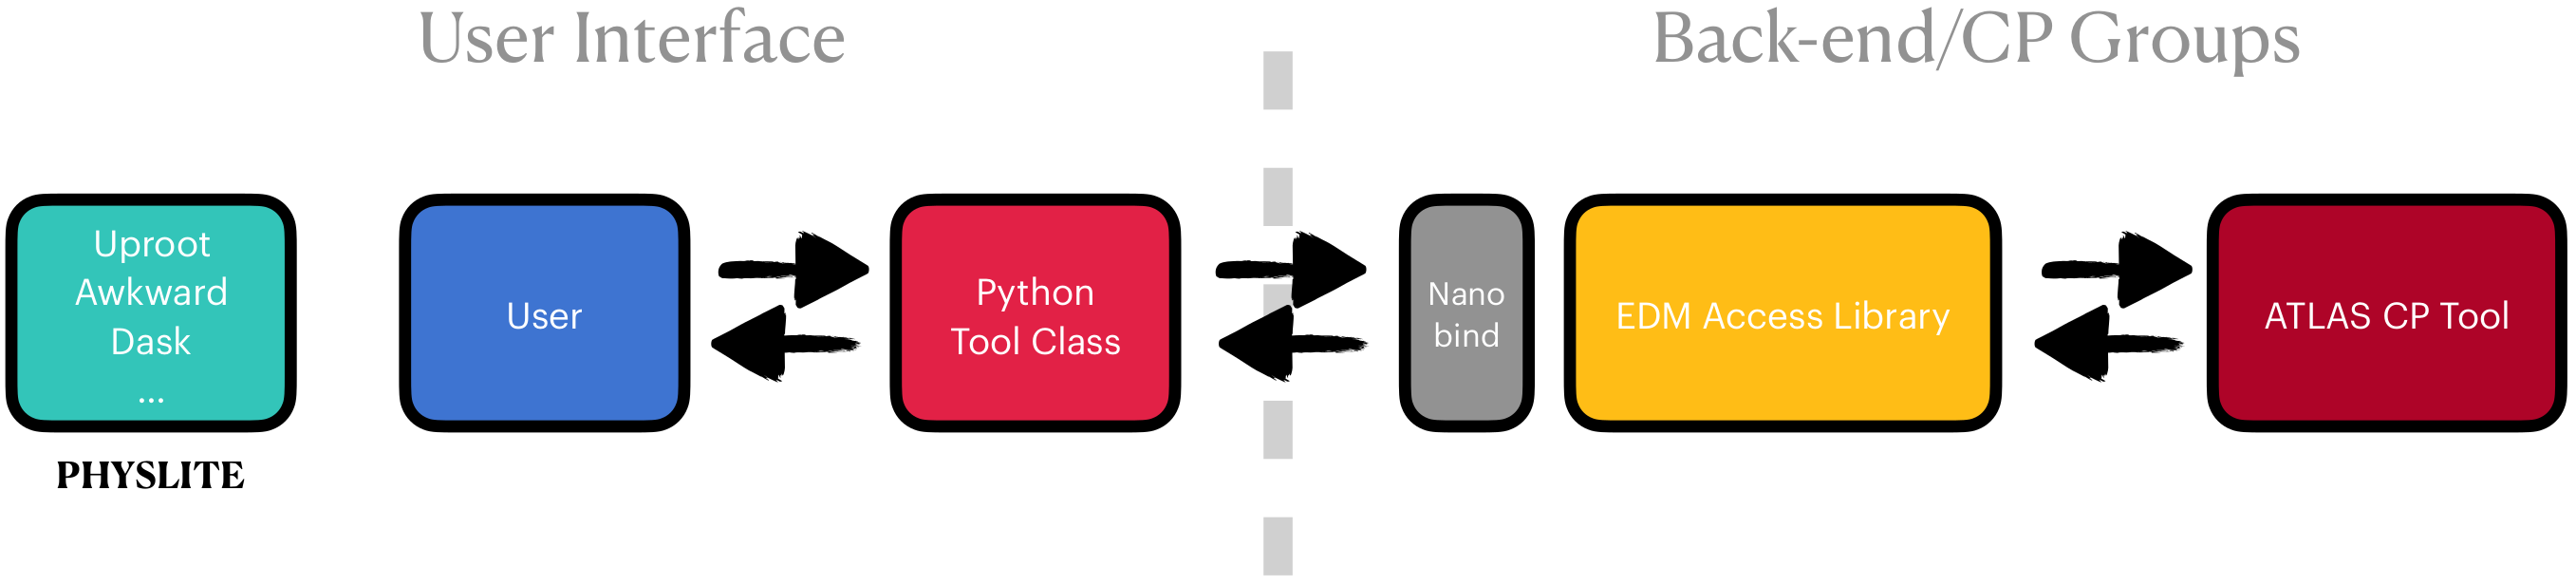
\includegraphics[width=\textwidth]{columnar_cp_tools_diagram.png}
    \caption{X~\cite{Vigl:ACAT_2024}.}
    \label{fig:columnar_cp_tools_diagram}
\end{figure}
